%!TEX root = ../thesis.tex

\chapter{Related Work}
\label{chapter_related_work}

% Typically, authors produce instructions manually. However,
The HCI and computer graphics communities have introduced novel technologies for authoring tutorials, including automatic generation methods and interactive editing tools.
%
In this chapter, we survey state-of-the-art techniques for generating instructions for both software applications (Section \ref{related_software}) and physical tasks (Section \ref{related_physical}).
%
Furthermore, today's tutorials are often offered within limited conventional media, such as static tutorials (print-outs or web) or videos. In recent years, interactive systems have shown versatile ways for users to review instructional content.
We will discuss the forms that instructions have taken in prior research, which will lead us to discuss shortcomings of tool support for creating and navigating tutorials.
%
Finally, in Section \ref{related_videos}, we review the methods of video analysis and playback to discuss how they support video-based interactions.

% -------------------------------------------

\section{Generating Instructions for Software Applications}
\label{related_software}

\subsection{Input Event Visualization}

% real-time
Studies have shown that visualizing input events during user operations can make software applications more learnable~\cite{Dixon:2010fb}. When viewing software instructions, visualizations can help learners anticipate where the cursor is moving, tell what actions are being performed, and locate activated UI components that may be otherwise hard to notice.

Input events that can be visualized range from low-level, application-agnostic input device events (e.g., mouse actions, cursor movements, or keyboard strokes) to higher-level, application-dependent information (e.g., menu selections or UI component changes).
%
Commercial tools such as Mouseposé\footnote{\url{http://www.boinx.com/mousepose}} and ScreenFlow\footnote{\url{http://www.telestream.net/screenflow}} visualize mouse events and keystrokes with special effects, e.g., drawing a circle around a mouse cursor (see Figure~\ref{fig:related_realtime}a). These tools capture input information (e.g., mouse position and event type) and render visualizations on top of the screen activities. This approach has been widely used by online video tutorial authors. However, it does not consider application context, which can be difficult for learners who want to follow specific instructions at a semantic level, such as observing text field completion or menu option selection.
% Some further enable video editing techniques, including zooming in/out  and panning.

To enhance UI components (e.g., a checkbox, button, or editable text field), Dixon \ea{}'s Prefab~\cite{Dixon:2010fb,Dixon:2011:CHP:1978942.1979086} modifies screen pixels in real-time by detecting target features, such as region corners. This semantic understanding of GUI elements enables component-based highlighting effects, such as afterglow~\cite{Baudisch:2006:PET:1166253.1166280} that visualizes user operations (see Figure~\ref{fig:related_realtime}b left). It also improves interactions by incorporating techniques like the Bubble Cursor~\cite{Grossman:2005:BCE:1054972.1055012}, a target-aware pointing method that suggests the nearest target (see Figure~\ref{fig:related_realtime}b right).

\begin{figure*}[t!]
  \centering
  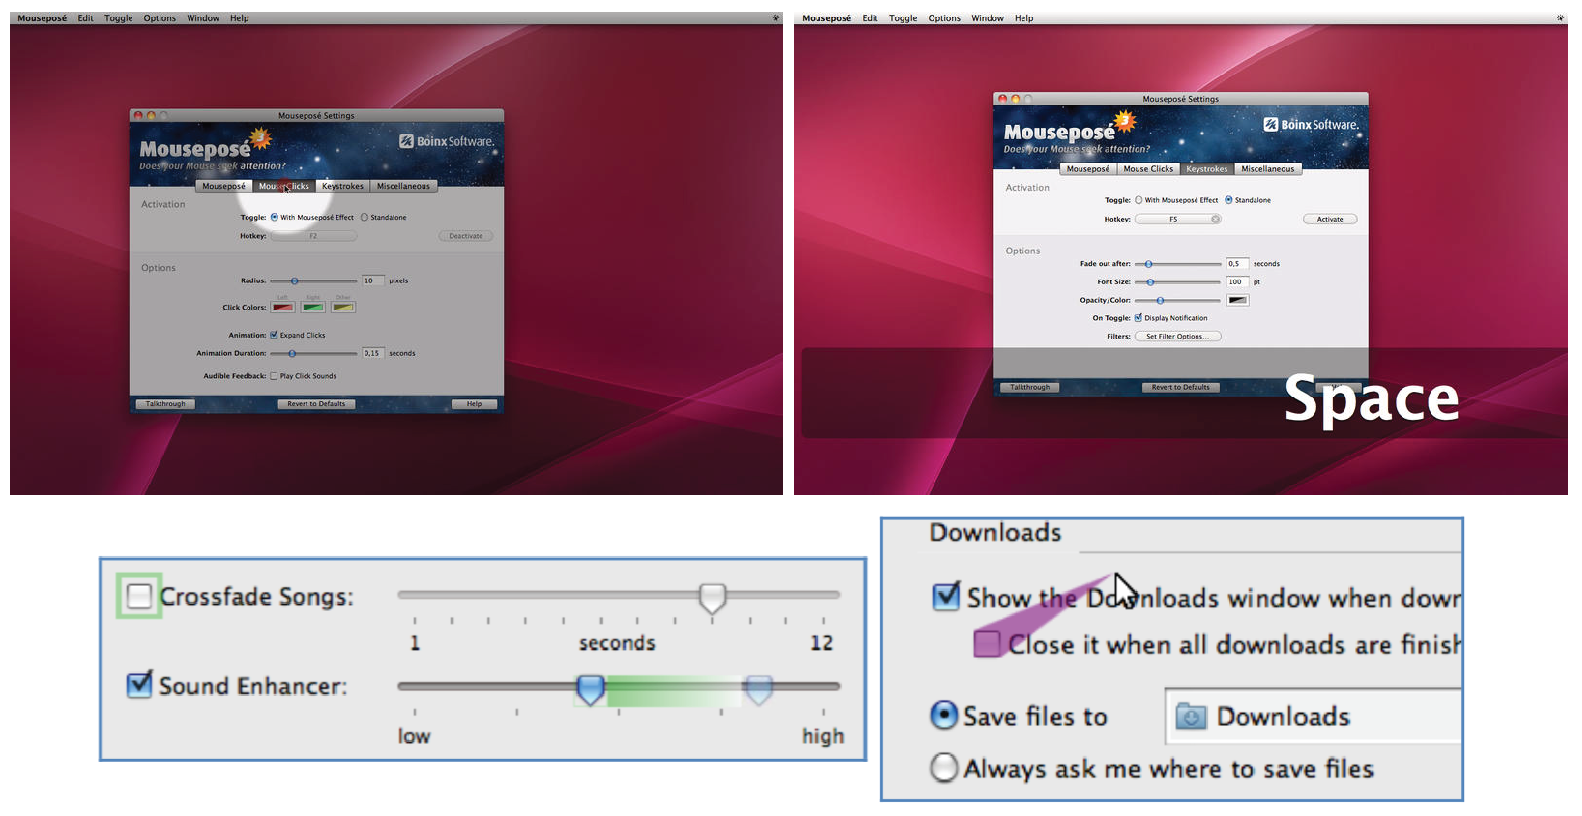
\includegraphics[width=0.7\textwidth]{\background/fig/realtime/realtime}
  \caption{Real-time visual enhancements to GUI applications are commonly used in instructional videos. Mouseposé highlights a mouse cursor (a, left) and displays keyboard input (a, right). Prefab~\cite{Dixon:2010fb} creates effects such as target-agnostic afterglow~\cite{Baudisch:2006:PET:1166253.1166280} (b, left) and target-aware cursor~\cite{Grossman:2005:BCE:1054972.1055012} (b, right) by identifying and reverse engineering UI components.}
  \label{fig:related_realtime}
\end{figure*}

% in screenshots
The methods above enable real-time visualization of input events when a user is interacting with an application or viewing playback of an application in use, which can be useful for following a video tutorial.
%
But to present events in a static tutorial, screenshot images are commonly annotated using different techniques in order to visualize continuous actions, such as navigating a menu from the root to a sub-panel. Applying motion arrows is a popular way to provide a sense of direction and start and end positions of mouse events.
%
Researchers have investigated automatic approaches that capture and visualize these types of events in representative screenshots from author demonstrations. Nakamura and Igarashi~\cite{Nakamura:2008:ASV:1449715.1449721} proposed a capturing and rendering system independent of specific GUI applications. Their system logs mouse events during a software demo, including mouse movement, dragging, and clicking. Operations are rendered as markers and arrows on screenshot images to present the linear event history (see Figure~\ref{fig:related_events}A).
%
Grabler \ea{}'s approach~\cite{Grabler:2009jj} further annotates a screenshot with bounding boxes and call-outs, which help learners identify parameters and specific functionality available in the interface (see Figure~\ref{fig:related_events}B).

\begin{figure*}[t!]
  \centering
  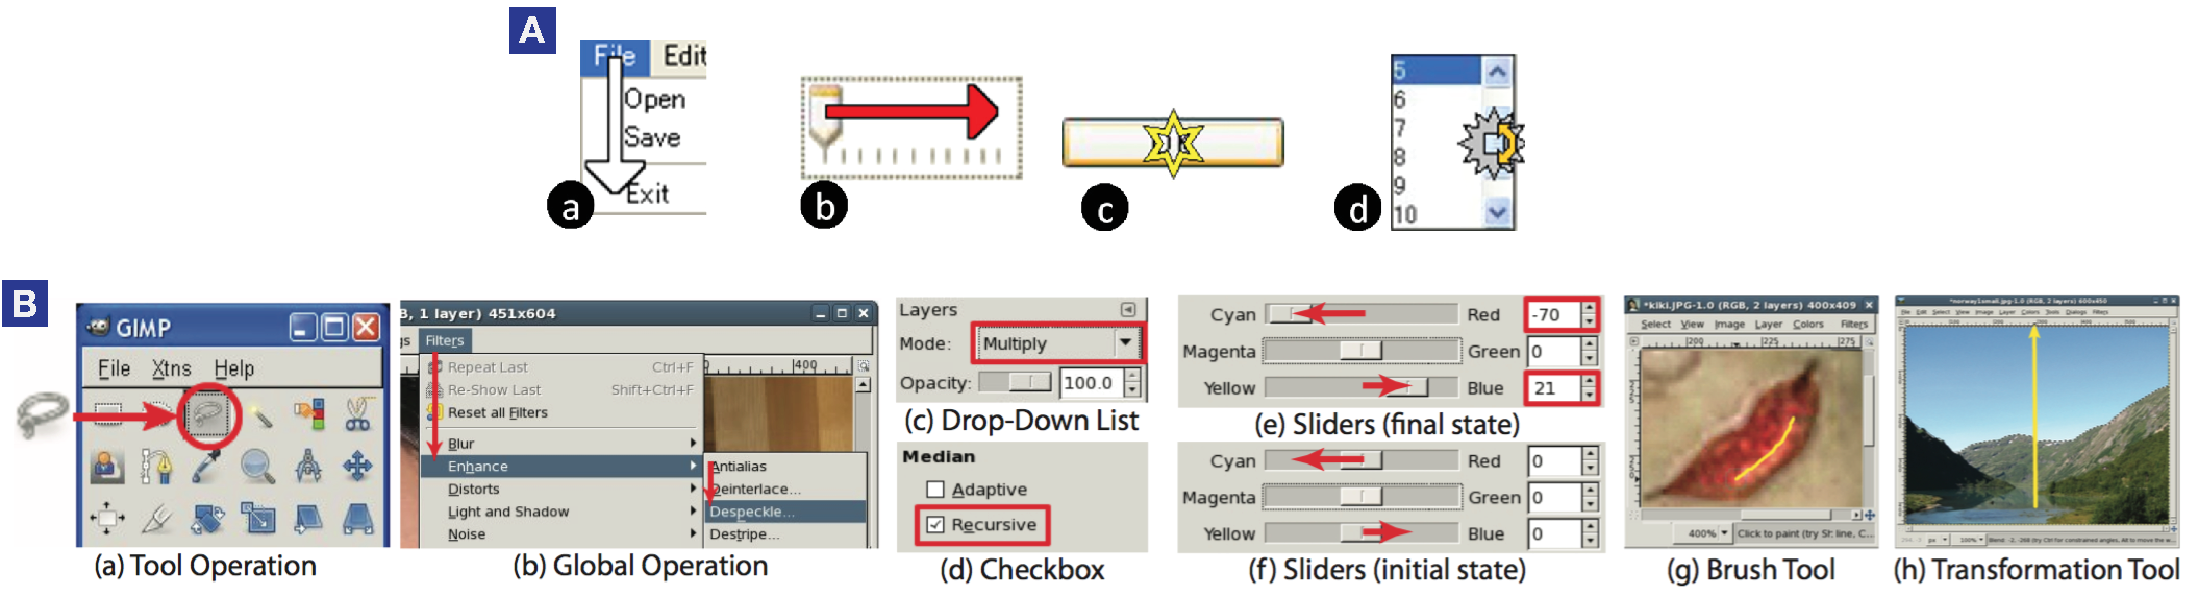
\includegraphics[width=\textwidth]{\background/fig/software_viz/software_viz}
  \caption{Examples where software operations are automatically rendered on top of application screenshots, including moving the mouse, dragging, clicking, and scrolling by Nakamura and Igarashi~\cite{Nakamura:2008:ASV:1449715.1449721} (A) and application-specific operations (a-b), parameter setting (c-f), and image manipulations (g-f) by Grabler \ea{}~\cite{Grabler:2009jj} (B).}
  \label{fig:related_events}
\end{figure*}

% summary
The systems we present adopt some of these successful techniques to enhance software instructions. By capturing event information at both input device and application levels, we visualize author operations differently based on how the learner is viewing instructions.
%
During \emph{video playback}, MixT shows mouse events and trails, and DemoWiz overlays glyphs and arrows to guide viewers from the current input event to the next.
%
Screenshot images in MixT's \emph{static} tutorials are annotated with mouse visualizations, such as highlighting a drop-down menu item that will be selected.

% -------------------

\subsection{Workflow Capture and Tutorial Generation}
In addition to visualizing input events, it is important to present the entire workflow in a tutorial and provide concise instructions.
%
Grabler \ea{}'s system~\cite{Grabler:2009jj} generates a step-by-step tutorial from an author's demonstration (see Figure~\ref{fig:related_static}). Generated tutorials include textual description, such as \iquote{Select the \textbf{path tool} from the \textbf{toolbar} to \textbf{create and edit paths}} from text templates, along with annotated images of user operations. Designed to guide image manipulation tasks, their system analyzes the application context, including facial features and outdoor scenes in manipulated images, to enhance instructions.
%
Such demonstration-based approaches have been applied to generate instructions for software that involves complicated manipulations or gestures, including 3D mesh construction~\cite{Denning:2011fy} and touch-based mobile applications~\cite{Wang:2014:EAC:2556288.2557407}.
%
Beyond logging input events during an author's demonstration, researchers have shown that workflows and user interface actions can be captured using computer vision by analyzing the pixels of desktop regions~\cite{Yeh:2009dh,Chang:2011vd} and existing screencast videos~\cite{Banovic:2012kd}.

\begin{figure*}[t!]
  \centering
  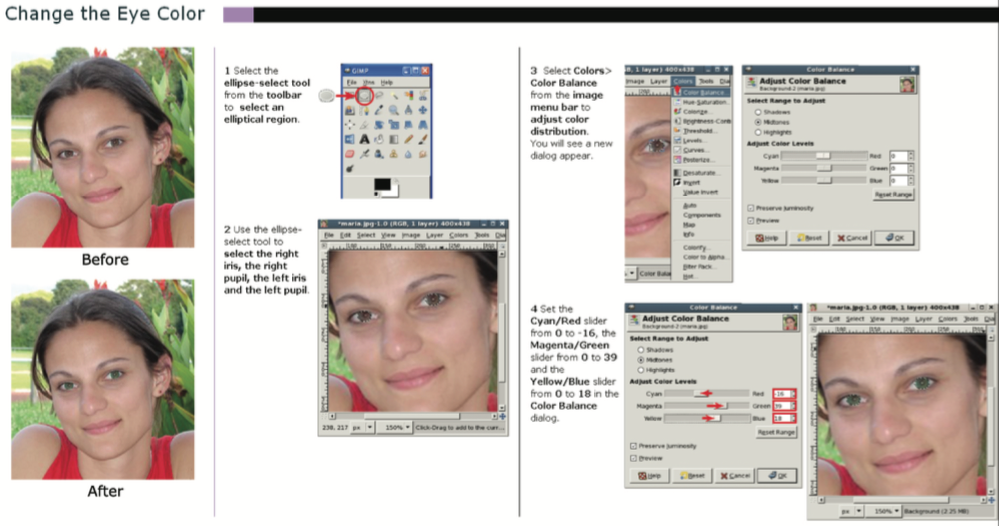
\includegraphics[width=0.75\textwidth]{\background/fig/related_static/grabler}
  \caption{A static tutorial automatically generated by Grabler \ea{}'s system~\cite{Grabler:2009jj}.}
  \label{fig:related_static}
\end{figure*}

With many tutorials to choose from, it can be useful for learners to have sophisticated ways to compare alternatives. To compare effects of individual operations in a workflow, showing a list of ``before'' and ``after'' thumbnails, video clips, and event timelines can be effective \cite{Grossman:2010jz}, as Chronicle demonstrated for image manipulation tasks (see Figure~\ref{fig:related_comparison}a).
%
When there are multiple workflows that produce similar results, side-by-side documents and a union graph, which shows the edit distance as a cluster view, can help learners choose the right workflow based on the operations each one uses~\cite{Kong:2012:DTR:2207676.2208549} (see Figure~\ref{fig:related_comparison}b).

\begin{figure*}[t!]
  \centering
  \includegraphics[width=\textwidth]{\background/fig/software_viz/related_comparison}
  \caption{Instructional systems that help learners compare image manipulations and similar tutorials using before and after images and event timelines by Grossman \ea{}~\cite{Grossman:2010jz} (a) and side-by-side documents by Kong \ea{}~\cite{Kong:2012:DTR:2207676.2208549} (b).}
  \label{fig:related_comparison}
\end{figure*}

% summary
These systems provided insights on 1) methods to automatically generate step-by-step tutorials and 2) workflow presentations serving different purposes.
%
Our MixT system draws on these past insights. It is build on top of a Photoshop plugin\footnote{Adobe labs. Tutorial Builder. \url{http://labs.adobe.com/technologies/tutorialbuilder/}} derived from Grabler \ea{}'s approach~\cite{Grabler:2009jj} to produce a step-by-step document with text descriptions of each workflow operation. We enhance the static tutorial format by embedding instructional video clips for each operation that can be interactively viewed.

The paradigm that these research projects explore opens a design space to create new tutorial formats for software applications. Our approaches show promise for helping learners effectively use tutorials. In recent years, researchers have shown that learners perform better when using responsive video tutorials~\cite{Nguyen:2015:MST:2702123.2702209} and learning-by-doing-activities~\cite{Kwon:2016:CEO:2858036.2858101}, than when using standard video or static instructions.

% -------------------

\subsection{In-Application Support}

The above methods introduce innovative ways for learners to review workflows and instructions. However, learners usually review these materials in an interface completely separate from the application they are learning to use. Learners might have to switch between the main application they are using and a separate set of instructions. This could widen the gulfs of execution and evaluation~\cite{Hutchins:1985:DMI:1453233.1453235} by making it more difficult for users to recall the actions to perform (\iquote{How do I perform the action that the instructions describe?}), or to evaluate whether they successfully followed instructions (\iquote{Am I doing this right as the instructions explain?}).

To reduce these gulfs, researchers have proposed another approaches to provide ``in-application'' assistance, often in real time, in a specific application context.
First, there has been a considerable amount of research devoted to offering interactive help to support learners comprehend the functionalities within the application.
%
Crystal~\cite{Myers:2006:AWW:1124772.1124832} enables software users to ask questions about why something did or did not occur in an application.
%
ToolClips~\cite{Grossman:2010wr} shows that video snippets can be embedded in application tooltips to explain specific functionality, which were shown to be seven times more effective than conventional tooltips for for users trying to complete unfamiliar tasks.

Second, interactive, step-by-step instructions can be integrated into an application in several forms:
%
To help software users identify specific UI components, tutorials can be shown via a translucent ``stencil,'' which visually directs a user's attention to relevant UI elements~\cite{Kelleher:2005:STD:1054972.1055047}.
%
By tracking a user's current actions, tutorials can be integrated with an application to provide indications of progress with check marks~\cite{Fernquist:2011:SRE:2047196.2047245}. Video tutorials can be programmed to automatically pause and play as users perform each step~\cite{Pongnumkul:2011ju}. Instructions can be captured from demonstrations as ``scripts'' to later guide step-by-step navigation within the interface~\cite{Bergman:2005:DocWizards} or shown as ambient help~\cite{Matejka:2011:AH:1978942.1979349}. In-application controls~\cite{Lieberman:2014:SML:2557500.2557543} and game elements~\cite{Li:2014:CGM:2556288.2556954, Dontcheva:2014:CCL:2556288.2557217} can further engage users in learning about the application.

Third, as tutorials are built for a broad community with many authors and learners, content can be dynamically updated by a community through user contributions~\cite{Lafreniere:2013ff,Matejka:2009:CCR:1622176.1622214, Bunt:2014:TPI:2556288.2557118}.

Our work focuses on authoring tools to create novel tutorial format designs, though it doesn't specifically focus on learning support. We see opportunities to provide the tutorials we generate as a form of in-application guidance. For example, a video clip from a MixT or DemoWiz tutorial could be automatically replayed when a system detects a slowdown of a learner's progress on a specific step. However, we do not claim to make a contribution in this direction.

% These projects show how effective instructional representations can assist learners in learning or executing tasks. Our goal is to further study new formats that incorporate advantages of several formats of multimedia, including images, text, and videos, and in turn enhancing the learning experience for a variety of tasks.

% * define ``automatic''
% Note: MixT tutorials are automatically rendered from manual demonstration, not automatically generated.

% To provide real-time assistance, it is important to recognize the user activities during a task performance. Several domains have been widely studied, including software operations, scene recognition, and object tracking in a physical world.

% -------------------------------------------

\section{Generating Instructions for Physical Activities}
\label{related_physical}

The above approaches to capture software demonstrations open the door to enable interactive tutorials that can respond to user progress. However, capturing and tracking user behavior in the physical world, rather than in software, remains challenging.
%
How can technologies track humans and objects in a space to support real-time feedback? What are the available authoring techniques to generate instructions for physical tasks?
%
This section discusses the challenges to approaches that researchers have taken from four perspectives, including tracking activities, authoring instructions, presenting guidance, and enabling interactive instruction following in the real world.

% -------------------

\subsection{Tracking Physical Activities}
To record activities and provide interactive feedback, a computer system needs to detect user operations and objects in real-time.
%
Computer vision techniques can automatically track specific physical targets shown in a video and enable novel interactions. This includes two types of targets:

\begin{itemize}
  \item \textbf{Tracking objects}. Instructional tasks often involve one or multiple objects, such as a ball in sports, utensils in cooking, and a variety of tools in DIY projects.
  Common techniques to track an object include:
  1) Tracking specific \emph{colors} or \emph{visual features} of pre-defined objects. Examples include tracking a fast-moving Ping-Pong ball for automatic camera control~\cite{Okumura:2011tr} or paper puppets for creating animations~\cite{Barnes:2008:VideoPuppetry}.
  Color and feature information can be supplemented with depth information, which could obtain a better understanding of the objects’ positions in the 3D world. Tracking objects in this way is useful to capture activities that involved object manipulations, such as block or toy assembly tasks~\cite{Gupta2012DuploTrack,Wu:2016:ARI:2856400.2856416} and 3D puppet control~\cite{held20123d};
  %
  2) Tracking \emph{motion-capture markers}. The most common method is to attach reflective markers to an object's surface. This enables accurate capturing of motions like an animator's continuous movements~\cite{Dontcheva:2003:LAC:1201775.882285}.
  %
  \item \textbf{Tracking humans}. Human activity can be tracked in many ways, often determined based on what activity is being monitored.
  Targets include \emph{faces} (e.g., to show a close-up of a speaker during video conferencing~\cite{Ranjan:2010}, to provide real-time camera control guidance when filming an interview~\cite{Carter:2010}, and to capture facial performances~\cite{Shi:2014:AAH:2661229.2661290,thies2016face}); \emph{hands} (e.g., to enable gestural control~\cite{taylor-siggraph2016} and camera control of a repair task~\cite{Ranjan:2008}); \emph{user movements} (e.g., to provide augmented content such as ambient information~\cite{Wilson:2012fb} and dancing~\cite{Anderson:2013:YEM:2501988.2502045}).
  %
  Motion capture markers can be used to track actors in addition to objects in professional filmmaking. However, since markers are visible in video recordings, visual effects (VFX) post-processing is necessary to hide them from the final rendering.
\end{itemize}

For many physical tasks, it's important to track both objects and humans. One example is reconstructing 3D scenes of athletes throwing basketballs~\cite{dou-siggraph2016}.
%
Some of these vision-based systems require a high-speed camera~\cite{Okumura:2011tr} or a RGB-D camera~\cite{Gupta2012DuploTrack,Wu:2016:ARI:2856400.2856416,held20123d,Wilson:2012fb,Anderson:2013:YEM:2501988.2502045,dou-siggraph2016}, while some require users to wear reflective markers~\cite{Ranjan:2008}.
%
Other non-vision tracking methods rely on sensors attached to an object or human, including GPS sensors~\cite{HexoDrone} and wireless radio frequency sensors~\cite{Nguyen:2016:ICR:2935620.2935632}. These are often used to track a moving target in a larger space, such as a flying drone.
%
Finally, if video content is difficult to be extracted into semantic information, crowdsourcing algorithms have been introduced to segment step-by-step videos with the help of online workers~\cite{Kim:2014:CSI:2611222.2556986}.

% summary
The detection mechanisms from these systems inspired us to design interactive systems that can react to an author's activities without requiring them to carry  a sensor. For example, Kinectograph and DemoDraw track authors' body parts using a Kinect sensor that is widely available to consumers.
%
However, tracking techniques to detect high-level task information, such as the \emph{intent} of a certain action, is still difficult to achieve. When automatic activity recognition is difficult, we include authors in the loop to annotate a task. DemoCut provides an annotation interface for describing high-level actions in DIY videos; DemoDraw provides a multi-modal interface to label continuous body movements.

% These methods usually require an expert defining heuristics of space regions or movement classifications ahead of time for the tracking program.

% -------------------

\subsection{Authoring Instructions for Real-World Tasks}

From current literature, we identified two major approaches to create instructions for physical tasks: model-based and demonstration-based.
%
A \emph{model-based} system analyzes the structure of an object or a task to generate instructions of how the object is constructed or the task is performed.
%
Early approaches by Feiner and Seligmann~\cite{feiner:1985:AEA:1299975.1300548,Seligmann:1991:AGI:127719.122732} considered communicative intent and rules of object manipulation to create effective illustrations from 3D models. Their automatically-generated diagrams showed that actions such as snapping latches can be effectively expressed by motion arrows and a cutaway view.
%
By analyzing object geometry and other attributes, Agrawala \ea{}'s~\cite{agrawala2003designing} system automatically renders step-by-step assembly instructions for furniture and toys (see Figure~\ref{fig:related_models}a).
%
Technical diagrams can also be generated, such as exploded views that explain mechanical assembly parts~\cite{li2008automated} and motion illustrations that describe how individual parts are operated~\cite{mitra2010illustrating}. Parts are often highlighted using colors, labeled with text; causal chain sequences of mechanical interaction can be shown as a list of highlighted figures, annotated with motion arrows (see Figure~\ref{fig:related_models}b).
%
Conversely, an existing technical document can be automatically analyzed and transformed into a 3D animation by parsing its parts, orientation, and visual annotations~\cite{Mohr:2015:RTD:2702123.2702490}.

\begin{figure*}[b!]
  \centering
  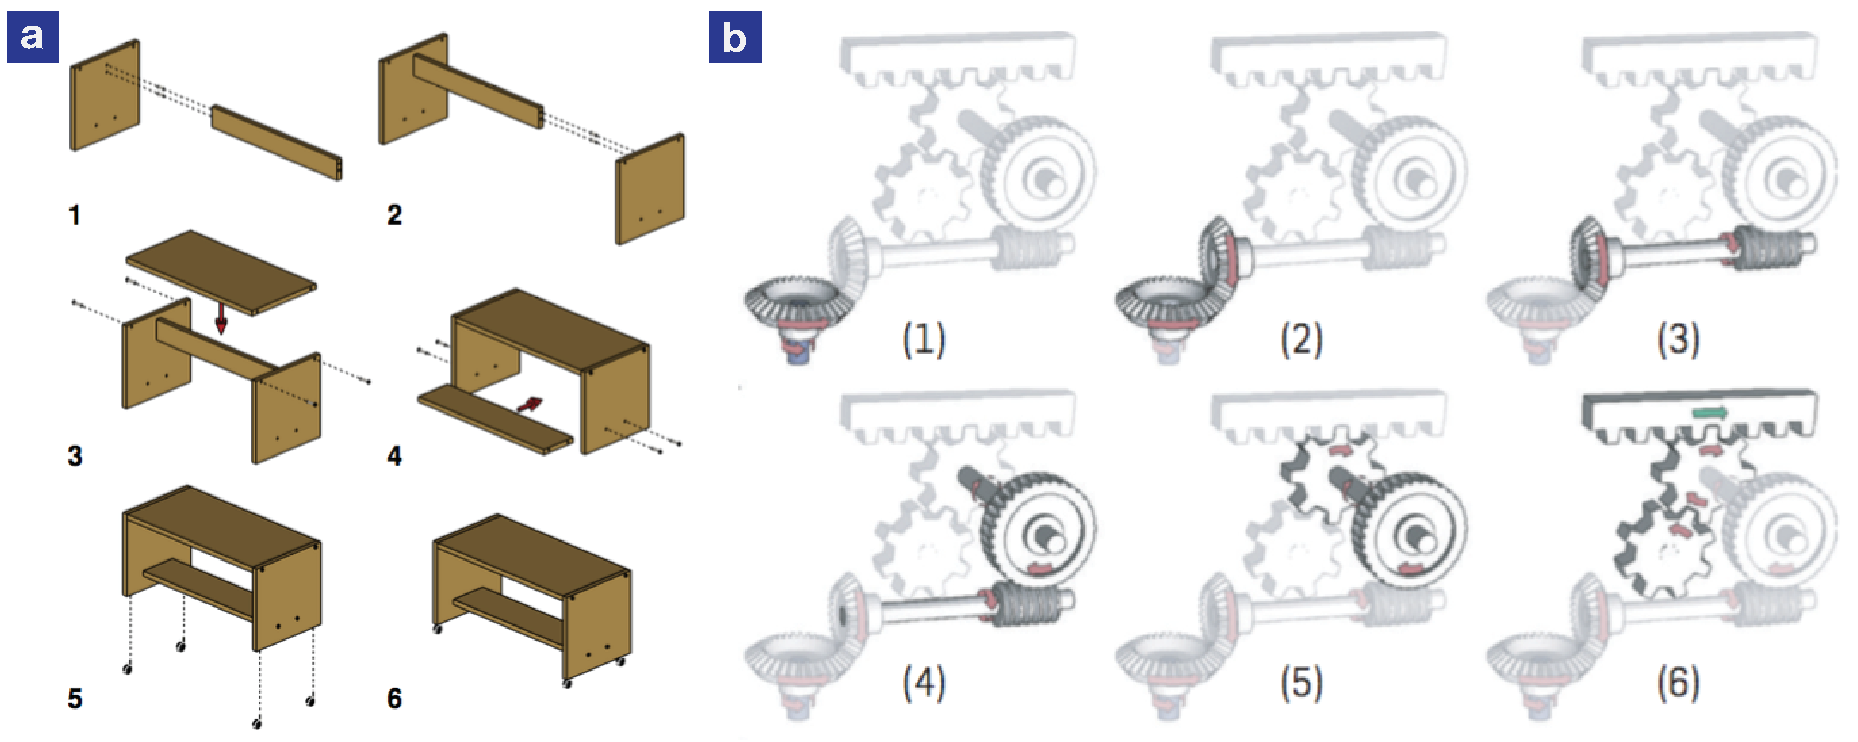
\includegraphics[width=0.8\textwidth]{\background/fig/model_generation/model_generation}
  \caption{Instructional diagrams can be automatically generated with a model-based approach, such as assembly instructions by Agrawala \ea~\cite{agrawala2003designing} (a) and causal chain sequences of mechanical interaction by Mitra \ea~\cite{mitra2010illustrating} (b).}
  \label{fig:related_models}
\end{figure*}

A \emph{demonstration-based} system records an author's physical demonstration of a workflow. The captured materials can be either automatically analyzed by the system or manually edited by an author to produce instructions.
%
One approach is to employ templates to help users capture sequences of distinct shots (e.g., Snapguide\footnote{\url{http://snapguide.com/}}) or provide a limited set of operations to record specific moments (e.g., adding or removing a part in a block-assembly task~\cite{Ranjan:2007,Gupta2012DuploTrack}).
%
Another approach is to provide a general-purpose interface to support authors produce multimedia materials during or after a demonstration, for example through an interface on a head-mounted video capture device~\cite{carter2015authoring}. For certain tasks, new recording devices need to be specially designed, such as an integrated device that includes an IR camera to capture a knitting process~\cite{Rosner:2008:SAK:1409635.1409682} and a turntable to record the building process of a DIY project~\cite{Tseng:2015:SPT:2771839.2771869}.

% summary
In this dissertation, we support a wide variety of physical tasks from craft to home repair and cooking where tracking user activities cannot be done completely automatically. Since the instructions produced in these domains are often highly creative and tailored to the author's style, we focus on the demonstration-based approach, which we feel is better capable of preserving the author's sensibilities.
%
Kinectograph and DemoDraw each allow authors to perform a physical demonstration in front of a camera, while capturing the activities given author's authoring decisions. DemoCut's annotation interface enables users to describe high-level, step-by-step instructions, such as tools and actions.

% -------------------

\subsection{Presenting Guidance}
To help learners follow instructions for physical tasks, we discuss how guidance has been displayed in the 3D world. There are four main approaches to present real-time guidance.

First, rich information can be shown via an \emph{external display} placed next to the work area. Applications in several domains adopt this method, in the domains of cooking~\cite{Uriu:2012:PRM:2207676.2207695} and block assembly tasks~\cite{Gupta2012DuploTrack,Wu:2016:ARI:2856400.2856416}. One challenge of external displays is that a learner may need to switch their attention often between the task and the instructions. To make instructions more easily accessible, Knibbe~\ea{}~\cite{Knibbe:2015:SMI:2817721.2817741} designed a table with an embedded display as a physical workspace that monitors, records, and assists users. In this way, workers could review the information on the table's surface while making a project.

\begin{figure*}[t!]
  \centering
  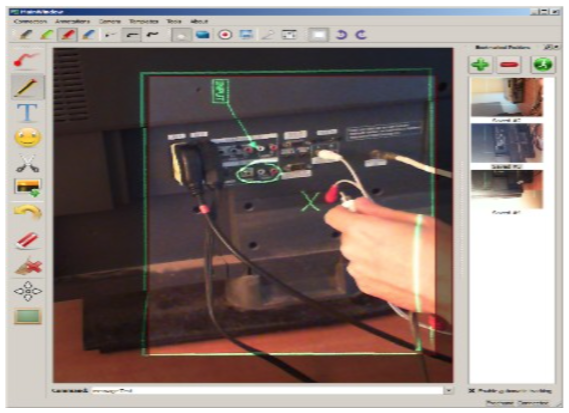
\includegraphics[width=0.4\textwidth]{\background/fig/ar/authoring}
  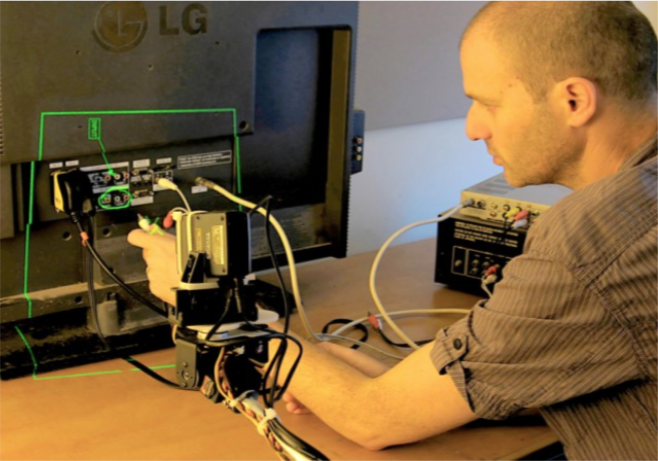
\includegraphics[width=0.41\textwidth]{\background/fig/ar/following}
  \caption{TeleAdvisor~\cite{Gurevich:2012ko} provides an authoring interface (left) for an instructor to guide a remote worker through a repair task (right).}
  \label{fig:related_teleadvisor}
\end{figure*}

\begin{figure*}[t!]
  \centering
  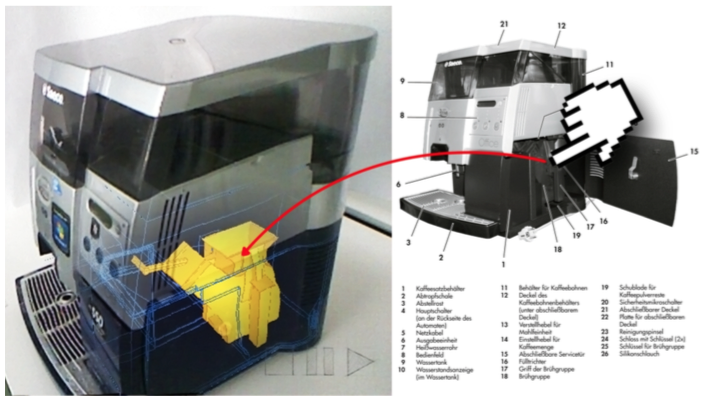
\includegraphics[width=0.55\textwidth]{\background/fig/ar/technical_document}
  \caption{Work by Mohr \ea{}~\cite{Mohr:2015:RTD:2702123.2702490} automatically analyzes a technical document and augments a machine with AR animations in 3D to help novices operate an unfamiliar machine.}
  \label{fig:related_ar_annotation}
\end{figure*}

Second, information can be \emph{overlaid on top of the work area} with a projector. Examples include remote repair tasks~\cite{Gurevich:2012ko} (see Figure~\ref{fig:related_teleadvisor} right), assembly tasks~\cite{Kirk:2006:CRG:1124772.1124951}, cooking~\cite{Ju:2001:CIC:634067.634227}, and learning to play the piano~\cite{Xiao:2016:IEI:2858036.2858577}.
%
For tasks such as dance movements, guidance can be shown on an augmented mirror that learners can reference~\cite{Anderson:2013:YEM:2501988.2502045}.
%
This method can effectively present instructions at a location that can be viewed most of the time by a learner as they perform the activities. However, this often requires a tailored indoor environment setup and a calibrated projector, which is difficult to integrate into most realistic settings where learners are doing these tasks.

Third, instructions can be \emph{displayed through a head-mounted device or mobile phone}. Researchers have built AR applications that provide visual highlights for machine maintenance~\cite{Henderson:2011ff,Mohr:2015:RTD:2702123.2702490} (see Figure~\ref{fig:related_ar_annotation}), enable interactive touring in a city~\cite{Feiner1997}, explain product functionalities~\cite{MagicLens}, and present dynamic user interfaces based on head orientation~\cite{Zhang:2014:HHO:2659766.2659773}.
%
Compared to other approaches that project information onto a publicly visible surface, this method allows learners to access information privately. Multiple users can interact with an augmented system at the same time. However, learners have to wear or carry a device, which might limit their mobility while performing a task, such as machine repair that requires both hands.

Last, for specific tasks, information can be conveyed \emph{directly via target objects}. Haptic feedback has shown to be useful to help learners follow steps for physical tasks, including sculpting~\cite{Zoran:2013:FFD:2470654.2481361,Agrawal:2015:PPS:2807442.2807505}, building multi-material assemblies~\cite{Schoop:2016:DSS:2851581.2892429}, and learning Frisbee~\cite{Solomon:2014:UTI:2540930.2540965}. Visual cues such as LED patterns on a device can direct user's attention to physical features they must interact with~\cite{Solomon:2014:UTI:2540930.2540965,Vasey:2016:HHR:2897839.2927404}.
%
This approach is task-specific and can be difficult to generalize to other task domains.

\subsection{Providing Activity-Based Guidance}
Finally, we discuss how assistive technologies track a learning process and support guidance based on learners' progress. For some specific tasks such as block assembly~\cite{Gupta2012DuploTrack,Wu:2016:ARI:2856400.2856416} and dancing~\cite{Anderson:2013:YEM:2501988.2502045}, learners' progress can be accurately tracked in 3D. This enables a tutorial system to provide real-time feedback about the learner's performance and what to do next, e.g., where to place the next block to the current model or suggested adjustment on a dance pose.
%
However, as we discussed earlier, tracking activities at the instruction level for real-world tasks can still be inaccurate. Therefore, the majority of systems supporting interactive physical guidance enable learners to navigate instructions.
%
For a pair learning scenario, a remote instructor can manually provide instructional input based on the learner's progress that he or she sees, such as highlighting a component for remote repair tasks~\cite{Gurevich:2012ko,Kirk:2006:CRG:1124772.1124951} (see Figure~\ref{fig:related_teleadvisor} left).

Our work focuses on designing tools for tutorial authors to create instructions from task demonstrations. DemoCut is designed for authoring instructions after capture time. Kinectograph provides a control interface on a tablet device for authors to carry and place in a space. DemoDraw's demonstration interface is similar to Anderson \ea{}'s~\cite{Anderson:2013:YEM:2501988.2502045} augmented mirror. But instead of overlaying instructions, we present a real-time render view of an author's movements via an external display placed in front of the user.

% -------------------------------------------

\section{Working with Videos}
\label{related_videos}

Research in video understanding has introduced new ways to work with videos. How should authoring tools help users record, organize, and edit necessary materials? What interaction techniques can help authors and viewers navigate one or more videos?
In this section, we review these questions and their answers briefly by considering current research tools designed to help users capture, edit, and navigate video.

% -------------------

\subsection{Tools for Capturing Video}
Tools that support video capture focus on these subtasks:

\subsubTitleBold{Shooting Suggestion}
Several research systems guide users at capture time to record higher-quality videos.
Real-time suggestions can help camera operators frame subjects (e.g., NudgeCam for interview videos~\cite{Carter:2010}) and provide suggestions for actors' performance (e.g., to speak louder or exaggerate a performance~\cite{Heer:2004ba,Davis:2003cu}). Shot suggestions can also be bootstrapped through user dialogs~\cite{Adams:2005}.
%
Other researchers recommend patterns from expert storytellers and common sense to help novice authors capture materials and develop a story structure~\cite{Barry:2003:MCC:957013.957152,Kim:2015:MSN:2702123.2702507}.

\subsubTitleBold{Automatic Camera Control}
Viewpoints of stationary cameras can be automatically determined based on heuristics at record time in order to track actor, area, or object~\cite{Ranjan:2008,Okumura:2011tr}.
%
In recent years, quadrotor cameras enable a wide range of trajectories to capture subjects from different viewing angles. Roberts and Hanrahan~\cite{Roberts:2016:GDF:2897824.2925980} proposed an authoring tool for authors to plan and preview a camera trajectory.
Some tools have enabled actors to control quadrotor cameras by using 3D gestures as they are being filmed~\cite{Cauchard:2015:DME:2750858.2805823,Pfeil:2013:EGM:2449396.2449429}.

% summary
We proposed Kinectograph prior to these systems of quadrotor camera control. A recent commercial system has included a similar feature to track a moving user~\cite{HexoDrone}, which is based on GPS information instead of specific body parts.

% -------------------

\subsection{Tools for Editing Video}
Tools that support video editing focus on these subtasks:

\subsubTitleBold{Annotation}
Researchers have investigated interactions that enable efficient, fluid annotation or labeling of video data. One example is the EVA system~\cite{Mackay:1989} that encourages authors to annotate materials at capture time. More recent interfaces accept pen input (e.g., VideoTater~\cite{Diakopoulos:2006vt}) and touch or gestural input~\cite{Sarkar:2016:SCC:2858036.2858199} for content-based annotations, such as tagging a subject in a video.

\subsubTitleBold{Storytelling}
When working with a repository of video clips, it can be challenging to compose a compelling story. Several new interaction techniques have been proposed to make it easier to explore story elements:
%
A storyline can be created non-linearly based on relevant characters, emotions, and themes of the current edited clips~\cite{Shen:2009:WNE:1518701.1518825}.
%
Tangible controllers with a specialized table interface can enable collaborative, non-linear editing~\cite{Bartindale:2012:STS:2207676.2207700,Bartindale:2016:TSS:2818048.2819929}.
%
Live authoring at capture time with a tablet device can allow an author to quickly organize clips and apply editing decisions~\cite{Freeman:2014:LLA:2611105.2557304}.

\subsubTitleBold{Editing}
Frame-based video editing is very time intensive, as it forces users to operate on very minute details. Editors can leverage \emph{metadata}, such as shot boundaries~\cite{Casares:2002dx} and transcripts~\cite{Berthouzoz:2012} that help users place cuts and transitions. This gives users higher-level editing operations at the shot level rather than the frame level.
%
Techniques of \emph{computer vision} and \emph{speech analysis} can automate certain visual effects, such as creating cinemagraphs~\cite{Bai:2012, Joshi:2012}, automatically editing lecture videos~\cite{Heck:2007}, creating zoomable tapestries and synopses~\cite{Barnes:2010,Pritch:2009vl}, and stabilizing shaky amateur videos~\cite{Liu:2011}.
%
Edits can take place during recording, such as switching to a close-up view of a person who is speaking~\cite{Ranjan:2010}.
%
When material like character animations can be reviewed in 3D, camera angles can be optimized to render a new video by analyzing the actor's motion data~\cite{assa2005action,assa2008motion}.
%
Finally, when video analysis is a matter of subjective taste, identifying salient frames or highlights can be outsourced to crowd workers~\cite{Bernstein:2011uj,Tang:2012:ECS:2207676.2208622}.

% summary
MixT, DemoCut, Kinectograph, and DemoDraw also use computer vision techniques for making automatic editing decisions. They differ from previous approaches in their focus on two particular application domains -- software and physical demonstration videos.
%
By focusing on a specific domain, MixT and DemoCut can make assumptions about the structure of the input and output video, such as the fact that there is a linear set of steps. DemoCut offers an authoring interface that makes it easier to create high quality instructional videos.
%
Kinectograph makes editing decisions (e.g., pan-and-tilt, zooming) based on an actor's body location in video frames.
%
DemoDraw includes a multi-modal interface where authors can annotate a recorded body motion using speech while physically performing movements.

% visual enhancement~\cite{Santosa:2013:DST:2470654.2466148}

% -------------------

\subsection{Tools for Navigating Video}
Video playback can be controlled by inferring user intention from their actions. For example, segments can be played back~\cite{Pongnumkul:2011ju} or speed can be modified~\cite{Cheng:2009:SUV:1518701.1518823} based on a user's actions in a software application.
%
Videos can be navigated at the content level beyond a linear timeline. For instance, subjects' movements can be visualized in a storyboard~\cite{goldman2006schematic} or continuous image mosaic~\cite{Teodosio:2005:SS:1047936.1047940}, and timelines can be navigated by manipulating a target in 2D~\cite{Dragicevic:2008:VBD:1357054.1357096,Goldman:2008:VOA:1449715.1449719,Karrer:2008:DDM:1357054.1357097} or 3D~\cite{Nguyen:2013:DMV:2470654.2466150}.
%
These techniques help viewers understand content flow and navigate videos, and have been applied to screencast videos~\cite{Denoue:2013:RDM:2451176.2451190,Nguyen:2015:MST:2702123.2702209}.
%
Canvases of video tiles and timelines~\cite{Al-Hajri:2014:VPH:2611105.2557106} or thumbnails~\cite{Matejka:2013:SIO:2470654.2466149} can make navigating long videos or sets of videos faster. Video digests can be an effective way for viewers to browse and skim video content~\cite{Pavel:2014:VDB:2642918.2647400}.
% Lecture videos~\cite{Tang:2006:DIU:1111449.1111523},

These novel forms of video navigation inspired us to help viewers navigate video content more effectively with our tools.
%
MixT supports per-step video navigation embedded in a static tutorial.
%
DemoWiz augments a screencast video with novel visualization to help users view the content.
%
DemoDraw renders a series of human movements as concise motion illustrations.

\subsection{Summary}
Our approaches take video as system \emph{input} (i.e., to track changes of salient UI components of screencast videos in MixT, DIY activities in DemoCut, and body movements in Kinectograph and DemoDraw), as well as \emph{output} (i.e., to offer interactive instructions with MixT's per-step video segments, DemoWiz's augmented screencast recording, DemoCut's concise video, and Kinectograph's instructor-focused video). We design user interfaces and algorithms for authors and learners to interact with video-based instructional content.
